\section{Logaritmus, logaritmická funkce}
\begin{definition}
    Nechť $a \in \mathbb R^+ \smallsetminus\left \{ 1 \right \} $. Pak inverzní
    funkci k exponenciální funkci $f:y=a^x$ nazýváme \textbf{logaritmickou
    funkcí} o základu $a$. Zapisujeme $f^{-1}: y=\log_a x.$
\end{definition}

\begin{figure}[ht!]
  \centering
  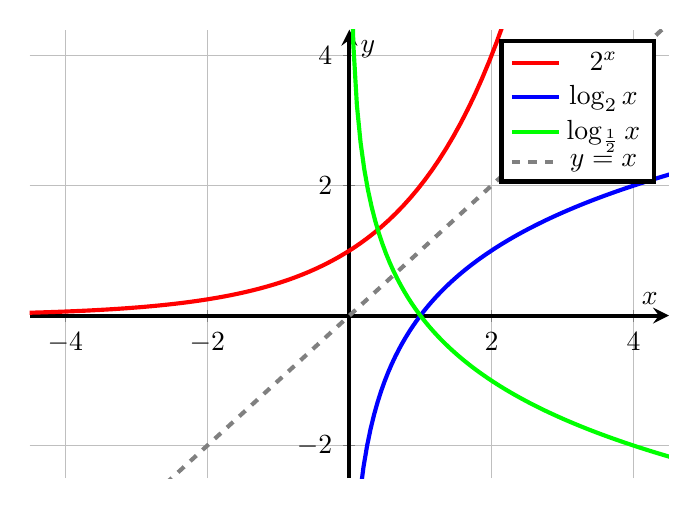
\begin{tikzpicture}
    \begin{axis}[
        axis lines = middle,
        xlabel = \(x\),
        ylabel = {\(y\)},
        line width=1.5pt,
        width=.8\textwidth,
        height=.6\textwidth,
        ymin=-2.5,
        ymax=4.4,
        xmin=-4.5,
        xmax=4.5,
        grid
    ]
    %Below the red parabola is defined
    \addplot [
        domain=-5:5,
        samples=100,
        color=red
    ]
    {2^x};
    \addlegendentry{\(2^x\)}

    \addplot [
        domain=0.1:5,
        samples=100,
        color=blue
        ]
        {ln(x)/ln(2)};
    \addlegendentry{\(\log_2 x\)}

    \addplot [
        domain=-0.1:5,
        samples=100,
        color=green
        ]
        {ln(x)/ln(0.5)};
    \addlegendentry{\(\log_\frac{1}{2}x\)}

    \addplot [
        domain=-5:5,
        samples=100,
        color=gray,
        dashed
        ]
        {x};
    \addlegendentry{\(y=x\)}

    \end{axis}
    \end{tikzpicture}
  \caption{Grafy funkcí $2x-1$ a $\frac{x+1}{2}$}
\end{figure}

\begin{veta}
    Nechť je dána logaritmická funkce $f:y=\log_a x$, $a \in \mathbb R^+ \smallsetminus
    \left \{ 1 \right \} $. Pak
    \begin{enumerate}[$i.$]
        \item $a>1: f$ je rostoucí,
       	\item $a < 1: f$ je klesající.
    \end{enumerate}
\end{veta}

\begin{definition}
    Nechť $f: y=\log_a x, a \in \mathbb R^+ \smallsetminus \left \{ 1 \right \}$ je
    logaritmická funkce a $x_0\in D(f).$ Pak číslo $f(x_0)$ nazýváme
    \textbf{logaritmem} čísla $x_0$ o základu $a.$
\end{definition}

\begin{pozn}
    Platí $\log_a b=c \iff a^c = b.$
\end{pozn}

\subsection*{Vlastnosti logaritmů}
\begin{veta}
    $\forall a \in \mathbb R^+ \smallsetminus \left \{ 1 \right \}:$
    \begin{enumerate}[$i.$]
        \item $\forall x \in \mathbb R^+: a^{\log_a x}=x$,
       	\item $\forall x \in \mathbb R: \log_a a^x=x$.
    \end{enumerate}
\end{veta}

\begin{proof}
    \,
    \begin{enumerate}[$i.$]
        \item $log_a x = r \iff a^r = x \iff a^{\log_a x}=x,$
       	\item $a^x = r \iff \log_a r=c \iff \log_a a^x = x.$ \qedhere
    \end{enumerate}
\end{proof}

\begin{veta}\label{zakl_reseni}
    $\forall a \in \mathbb R^+ \smallsetminus \left \{ 1 \right \},
    \forall x_1, x_2\in \mathbb R^+: \log_a x_1 = \log_a x_2 \iff x_1 = x_2$.
\end{veta}

\begin{veta}
    $\forall a,b,c\in \mathbb R^+, a\ne 1, b\ne 1:$
    \begin{enumerate}[$i.$]
        \item $\log_a b \cdot \log_b c = \log_a c,$
       	\item $\log_a b \cdot \log_b a = 1.$
    \end{enumerate}
\end{veta}

\begin{proof}
    \,
    \begin{enumerate}[$i.$]
        \item
            $\log_a b = r \iff a^r = b,$ \\
            $\log_b c = s \iff b^s = c,$ \\
            $\log_a c = t \iff a^t = c,$ \\
            $c =b^s=\left ( a^r \right )^s,$ \\
            $c = a^t,$ \\
            $a^{rs} = a^t \implies rs = t \implies \log_a b \cdot \log_b c = \log_a c,$
        \item $\log_a b\cdot \log_b a = \log_a a = 1.$\qedhere
    \end{enumerate}
\end{proof}

\begin{veta}
    $\forall a,b,c\in \mathbb R^+, a\ne 1, b\ne 1:$
    \begin{enumerate}[$i.$]
        \item $\log_b c = \frac{\log_a c}{\log_a b},$
       	\item $\log_a b = \frac{1}{\log_b a}.$
    \end{enumerate}
\end{veta}

\begin{veta}
    $\forall a \in \mathbb R^+ \smallsetminus \left \{ 1 \right \}  , \forall x \in \mathbb R^+:$
    \begin{enumerate}[$i.$]
        \item $\log_{\frac{1}{a}} x = -\log_a x,$
       	\item $\log_a \frac{1}{x} = -\log_a x.$
    \end{enumerate}
\end{veta}

\begin{proof}
    \,
    \begin{enumerate}[$i.$]
        \item Nechť $\log_{\frac{1}{a}} x = r, \log_a x = s.$ Pak
        $\left ( \frac{1}{a} \right )^r = a^s,$ tedy $a^{-r}=s,$ takže $r=-s$.
        Odtud $\log_{\frac{1}{a}} x = -\log_a x.$
       	\item Nechť $\log_{\frac{1}{a}} x = r, \log_a x = s.$ Pak
        $x = \frac{1}{a^r}=a^s,$ obdobně $r=-s,$ takže $\log_a \frac{1}{x}=
        -\log_a x.$\qedhere
    \end{enumerate}
\end{proof}

\begin{veta}
    $\forall a \in \mathbb R^+ \smallsetminus \left \{ 1 \right \}, \forall x,y \in \mathbb R^+
    ,\forall r \in \mathbb R:$
    \begin{enumerate}[$i.$]
        \item $\log_a (xy)=\log_a x + \log_a y,$
       	\item $\log_a \left ( \frac{x}{y} \right ) = \log_a x - \log_a y,$
       	\item $\log_a x^r = r\cdot \log_a x.$
    \end{enumerate}
\end{veta}

\begin{proof}
    Ve všech případech předpokládejme $\log_a x = s \iff x = a^s,
    \log_a y = t \iff y = a^t.$
    \begin{enumerate}[$i.$]
        \item $xy = a^sa^t=a^{s+t},$\\
        $\log_a (xy) = \log_a (a^{s+t}) = s+t=\log_a x + \log_a y,$
       	\item $\log_a \left ( \frac{x}{y} \right )  = \log_a
        \left ( \frac{a^s}{a^t} \right ) =\log_a \left ( a^{s-t} \right ) =
        s-t,$
       	\item $\log_a x^r = \log_a \left [ \left ( x^s \right )^r  \right ] =
        \log_a a^{rs}=rs=r\cdot \log_a x.$\qedhere
    \end{enumerate}
\end{proof}

\begin{definition}
    Nechť $x\in \mathbb R^+.$ \textbf{Dekadickým logaritmem} čísla $x$ rozumíme
    jeho logaritmus o základu 10. Zapisujeme $\log x.$
\end{definition}

\begin{veta}\label{mantisa}
    Nechť $m\in \mathbb R^+.$ Pak platí
    $$\log m = \log m_1 + c,$$
    kde $\log m_1 \in \left < 0,1 \right >, c \in \mathbb Z,$ a toto vyjádření
    je jednozančné.
\end{veta}

\begin{proof}
    $\log m = \log \left ( m_1\cdot 10^c \right ) = \log m_1 + \log 10^c
    = \log m_1 + c$
\end{proof}

\begin{definition}
    Číslo $\log m_1$ z věty \ref{mantisa} nazýváme \textbf{mantisou} a číslo
    $c$ \textbf{charakteristikou} čísla $\log m.$
\end{definition}

\begin{definition}
    Nechť $x \in \mathbb R\smallsetminus\left \{ 1 \right \}. $ \textbf{Přirozeným logaritmem} čísla $x$
    rozumíme logaritmus o základu $e$. Zapisujeme $\ln x.$
\end{definition}

\begin{definition}
    (Ne)rovnice, ve které se vyskytuje logaritmus, se nazývá \textbf{Logaritmická (ne)rovnice}.
    Řešíme je na základě věty \ref{zakl_reseni}.
\end{definition}

\begin{veta}
    $\forall a \in \mathbb R^+ \smallsetminus \left \{ 1 \right \} , \forall x_1, x_2
    \in \mathbb R:$
    \begin{enumerate}[$i.$]
        \item pro $a>1:a^{x_1}<a^{x_2}\iff x_1 < x_2,$
       	\item pro $a \in (0,1): \log_a x_1 < \log_a x_2 \iff x_1 > x_2.$
    \end{enumerate}
\end{veta}

\begin{veta}
    $\forall a \in \mathbb R^+ \smallsetminus \left \{ 1 \right \} , \forall x_1, x_2
    \in \mathbb R^+:$
    \begin{enumerate}[$i.$]
        \item pro $a>1:\log_a x_1 < \log_a x_2 \iff x_1 < x_2$,
       	\item pro $a\in (0,1): \log_a x_1 < \log_a x_2 \iff x_1 > x_2.$
    \end{enumerate}
\end{veta}
